% =============================================================================
%  s01_intro.tex — Sección 1: Introducción / Planteamiento del problema
%  Sustituye \lipsum con tu contenido real.
% =============================================================================

\section{Introducción}

% ── Frame: Contexto ───────────────────────────────────────────────────────────
% NOTA \pause: revela bullets uno a uno durante la presentación en vivo,
%   pero genera páginas PDF duplicadas. Descomenta solo si presentas en proyector.
\begin{frame}{Definición Multidimensional de la Movilidad Sustentable}
    \begin{block}{Un Enfoque Integrador}
        La movilidad urbana sustentable trasciende la eficiencia técnica para consolidarse como un enfoque multidimensional que equilibra los ejes \textbf{social, económico y ambiental} \cite{RamirezPacheco2025}.
    \end{block}
    
    \begin{itemize}
        \item \textbf{Ciudad Habitable vs. Ciudad Productiva:} Búsqueda de un equilibrio entre el dinamismo económico y la calidad de vida urbana \cite{RedalycPeaton}.
        \item \textbf{Sostenibilidad a Largo Plazo:} Garantizar que las necesidades de traslado actuales no comprometan la viabilidad de las generaciones futuras \cite{SEDATU2023}.
        \item \textbf{Eficiencia Energética:} Reducción de externalidades negativas y priorización de tecnologías de bajo impacto ambiental.
    \end{itemize}
\end{frame}


% 1.2. El Cambio de Paradigma
\begin{frame}{El Cambio de Paradigma: Del Transporte a la Movilidad}
    \begin{itemize}
        \item \textbf{Paradigma Tradicional (Transporte):} Centrado en la gestión del flujo vehicular, la capacidad de carga vial y la velocidad del automóvil particular \cite{RedalycPeaton}.
        \item \textbf{Paradigma Contemporáneo (Movilidad):} Enfoque antropocéntrico basado en la \textbf{accesibilidad de las personas} y su interacción con el entorno urbano \cite{ramirez2025analisis}.
    \end{itemize}

    \begin{exampleblock}{Visión del Urbanismo Posmoderno}
        El éxito de un sistema de movilidad no se mide por el volumen de vehículos, sino por la capacidad de los ciudadanos para acceder a las oportunidades de la ciudad de forma segura y eficiente.
    \end{exampleblock}
\end{frame}

% 1.3. Marco Legal del Artículo 4° Constitucional
\begin{frame}{Marco Legal: Artículo 4° Constitucional en México}
    \begin{block}{Derecho Humano a la Movilidad (Reforma 2020)}
        \textit{"Toda persona tiene derecho a la movilidad en condiciones de seguridad vial, accesibilidad, eficiencia, sostenibilidad, calidad, inclusión e igualdad"} \cite{ConstitucionMex}.
    \end{block}

    \begin{itemize}
        \item \textbf{ENAMOV 2023-2042:} Instrumento rector derivado del mandato constitucional para alinear la política pública nacional \cite{SEDATU2023}.
        \item \textbf{Jerarquía de Movilidad:} Obligatoriedad de priorizar a los usuarios más vulnerables (peatones y ciclistas) en el diseño de las vías urbanas.
        \item \textbf{Justicia Socioespacial:} Reducción de brechas de desigualdad en el acceso a servicios básicos mediante el transporte público.
    \end{itemize}
\end{frame}

\begin{frame}{Sustento Visual: Jerarquía y Eficiencia del Espacio}
  \begin{columns}[T]
    \begin{column}{0.48\textwidth}
      \centering
       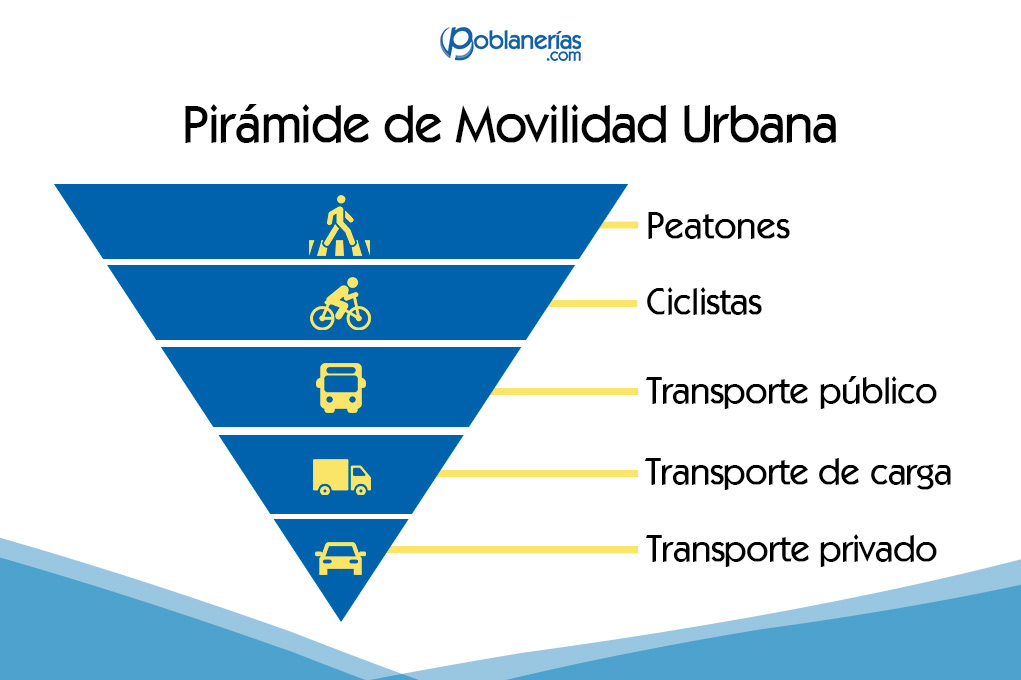
\includegraphics[width=\textwidth, height=3.8cm, keepaspectratio]{img/Piramide-de-Movilidad-Urbana.jpg}
      {\small \textbf{Pirámide de Movilidad:} Priorización oficial que sitúa al peatón y ciclista en la cúspide según la ENAMOV \cite{SEDATU2023}.}\\[0.05cm]
      \fuentefigura{NOM-004-SEDATU-2023 \cite{NOM004}.}
    \end{column}
    \begin{column}{0.48\textwidth}
      \centering
       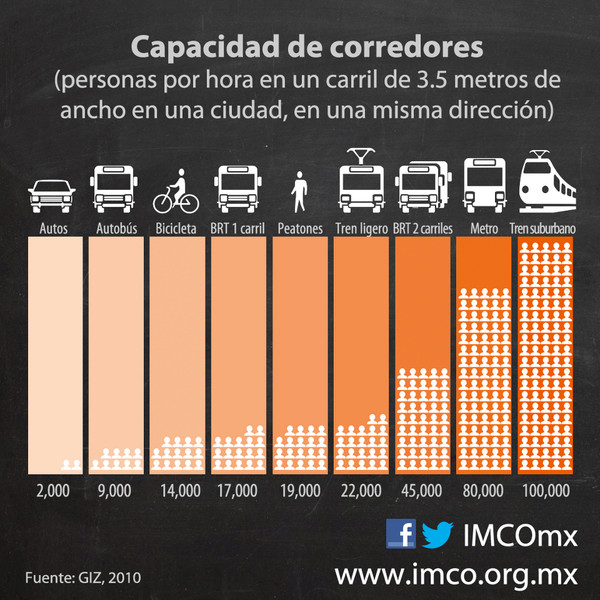
\includegraphics[width=\textwidth, height=3.8cm, keepaspectratio]{img/Capacidad.png}
      {\small \\ \textbf{Capacidad por modo:} Comparativa de personas transportadas\cite{ITDP_Espacio}.}\\[0.05cm]
      \fuentefigura{Adaptado de ITDP México \cite{ITDP_Espacio}.}
    \end{column}
  \end{columns}
\end{frame}


% 1.4. Reflexión Crítica: La Metáfora de la Higuera de Sylvia Plath
\begin{frame}{Reflexión Crítica: La Metáfora de la Higuera de Sylvia Plath}
    \begin{columns}
        \begin{column}{0.5\textwidth}
            \begin{itemize}
                \item \textbf{El Sistema Radial:} Obliga al usuario a elegir una sola "rama" (el centro), saturando los nodos centrales.
                \item \textbf{Saturación Sistémica:} Al no existir alternativas transversales, las opciones de accesibilidad en la periferia "se marchitan".
            \end{itemize}
        \end{column}
        \begin{column}{0.5\textwidth}
            \begin{alertblock}{Propuesta de Tesis (VFT)}
                Es imperativo crear \textbf{"ramas transversales"} (Corredores Anillares) que intercepten los flujos y preserven la viabilidad de todas las opciones de movilidad en la ZMVM.
            \end{alertblock}
        \end{column}
    \end{columns}
\end{frame}